\documentclass[12pt]{article}
\usepackage[breaklinks=true]{hyperref}
\usepackage[margin=0.75in]{geometry}

\usepackage{graphicx}
\usepackage{color}
\usepackage{amsmath}

\definecolor{pblue}{rgb}{0.13,0.13,1}
\definecolor{pgreen}{rgb}{0,0.5,0}
\definecolor{pred}{rgb}{0.9,0,0}
\definecolor{pgrey}{rgb}{0.46,0.45,0.48}

\usepackage{listings}
\lstset{language=Java,
  showspaces=false,
  showtabs=false,
  tabsize=2,
  breaklines=true,
  showstringspaces=false,
  breakatwhitespace=true,
  numbers=left,
  commentstyle=\color{pgreen},
  keywordstyle=\color{pblue},
  stringstyle=\color{pred},
  basicstyle=\ttfamily,
  frame=single,
  moredelim=[il][\textcolor{pgrey}]{$$},
  moredelim=[is][\textcolor{pgrey}]{\%\%}{\%\%}
}

\title{Final Exam Prep}
\author{
	Melvyn Ian Drag
}
\date{\today}


\begin{document}
\maketitle

\begin{abstract}
Prepare for exam
\end{abstract}

\section{Final Exam}
Set your path to point to your compiler and JVM. Then compile a simple program.

\subsection{What is a PATH}
The Path/PATH is an `environment variable'. It's a variable that tells your
operating system where to look for various programs when you try to run them.
For example, on the command line, when you type `javac' your computer needs to
know where `javac' is saved. This is why we have to put it in our PATH.

\subsection{Set Up Your Path}
On windows you typically set your path as shown in figure \ref{setenvvar} and
figure \ref{pathwindows}.

\begin{figure}[h]
  \centering
    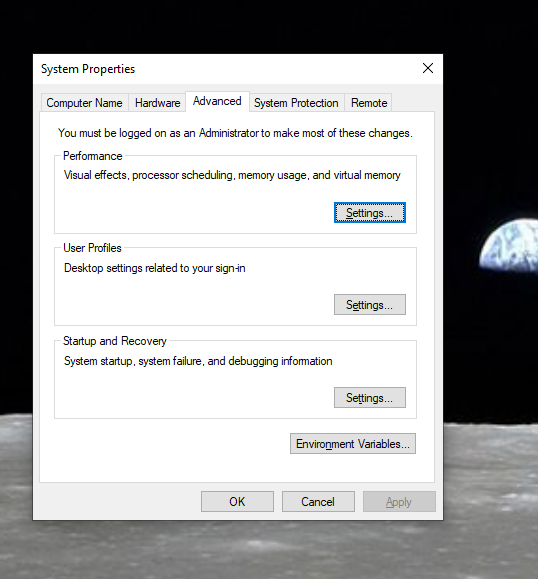
\includegraphics[width=0.9\textwidth]{Images/windowssetenv.PNG}
  \caption{Click on `Environment Variables'.}
	\label{setenvvar}
\end{figure}

\begin{figure}[h]
  \centering
    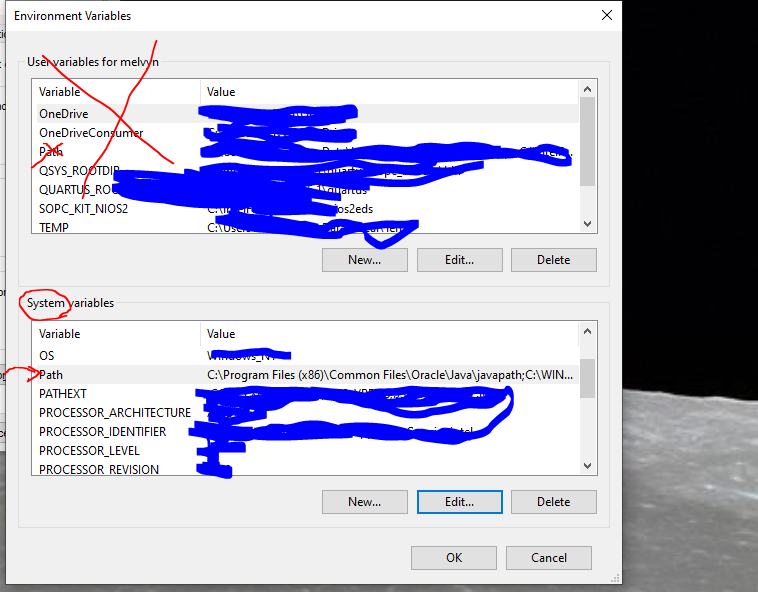
\includegraphics[width=0.9\textwidth]{Images/path0.PNG}
  \caption{Modify what is in your PATH. Crossing stuff out in case there is
anything you might use to hack me or whatever, this is my home PC.}
	\label{pathwindows}
\end{figure}

Unfortunately, for this class we don't have administrator access to our lab
computers, so we need a work around. To this end, we have used the 'git bash'
shell instead of the windows `cmd' shell. This gives us a small Linux-like
environment in which we can modify the PATH using Linux techniques. To set your
path in Linux you need to modify you path in a file called `\~{}/.bashrc'

You need to find where \textit{java} and \textit{javac} are installed on your
computer. For me they are in the location showing in figure
\ref{myjavalocation}.

\begin{figure}[h]
  \centering
    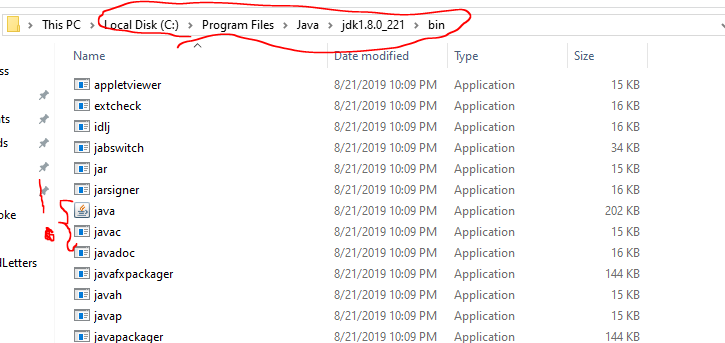
\includegraphics[width=0.9\textwidth]{Images/javaPrograms.PNG}
  \caption{ Install location of my java and javac}
	\label{myjavalocation}
\end{figure}

Then I update my .bashrc file as is shown in figure \ref{mybashrc}.

\begin{figure}[h]
  \centering
    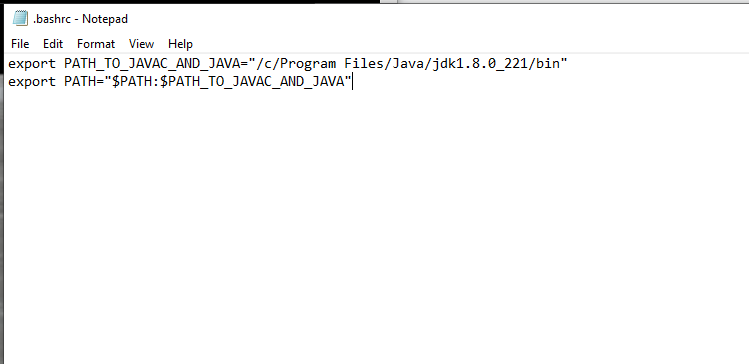
\includegraphics[width=0.9\textwidth]{Images/my_bashrc.PNG}
  \caption{my bashrc file}
	\label{mybashrc}
\end{figure}

Make sure you create a .bashrc file just like mine - the only thing you should
hcnage is the path to where your java bin directory is. Everything else must be
excatly the same! This will be saved in your home directory. This is something
like

\begin{verbatim}
C:\Users\NJCU_ID
\end{verbatim}

Note where and how I save my file in figure \ref{savebashrc}.

\begin{figure}[h]
  \centering
    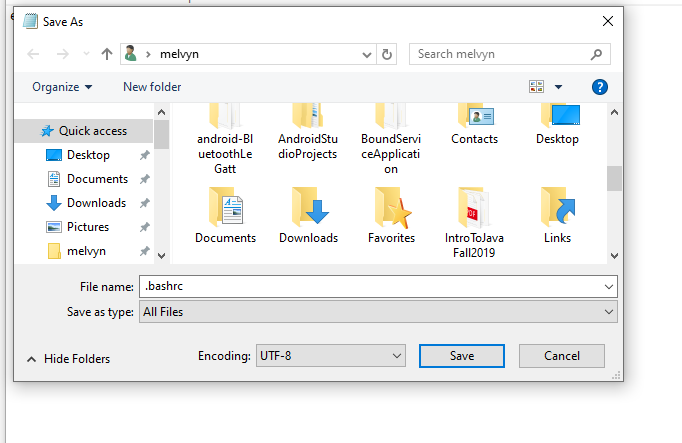
\includegraphics[width=0.9\textwidth]{Images/bashrcSaving.PNG}
  \caption{where to save .bashrc}
	\label{savebashrc}
\end{figure}

\begin{center}
{\LARGE Note that the file is called .bashrc, not bashrc. Not bashrc.txt. Not
\_bashrc.  Make sure the file is named correctly.}
\end{center}

We are only using gitbash in this class instead of cmd because a) we need to get
around IT restrictions b) I know linux and git bash has some linux
functionality that I know well, so I can confidently teach it to you. Generally
you would modify your windows environment variables as shown in the beginning of
this section.

When you have successfully configured your .bashrc and open gitbash you might
see a warning as demonstrated in figure \ref{errorisokay}.

\begin{figure}[h]
  \centering
    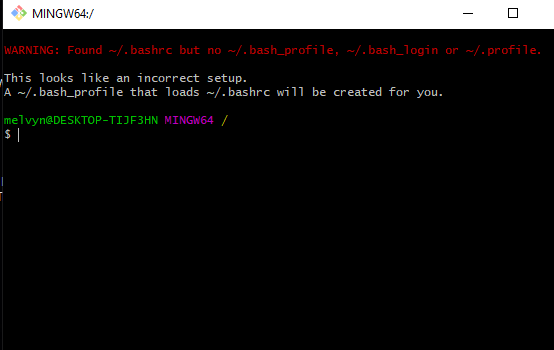
\includegraphics[width=0.9\textwidth]{Images/errorIsOkay.PNG}
  \caption{You might see this warning. Ignore it.}
	\label{errorisokay}
\end{figure}

Then type the `cd' command followed by `cat .bashrc'. You should see something
like what is shown in figure \ref{cat}.

\begin{figure}[h]
  \centering
    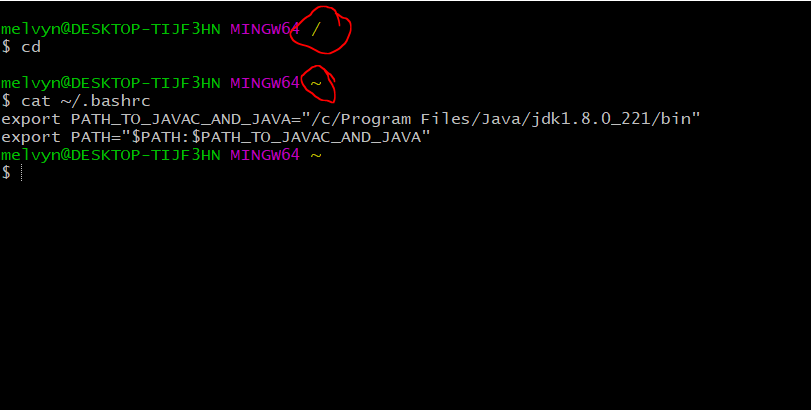
\includegraphics[width=0.9\textwidth]{Images/catbashrc.PNG}
  \caption{checking the contents of .bashrc}
	\label{cat}
\end{figure}

At this point javac should be working, so type javac in git bash as shown in
figure \ref{javac}.

\begin{figure}[h]
  \centering
    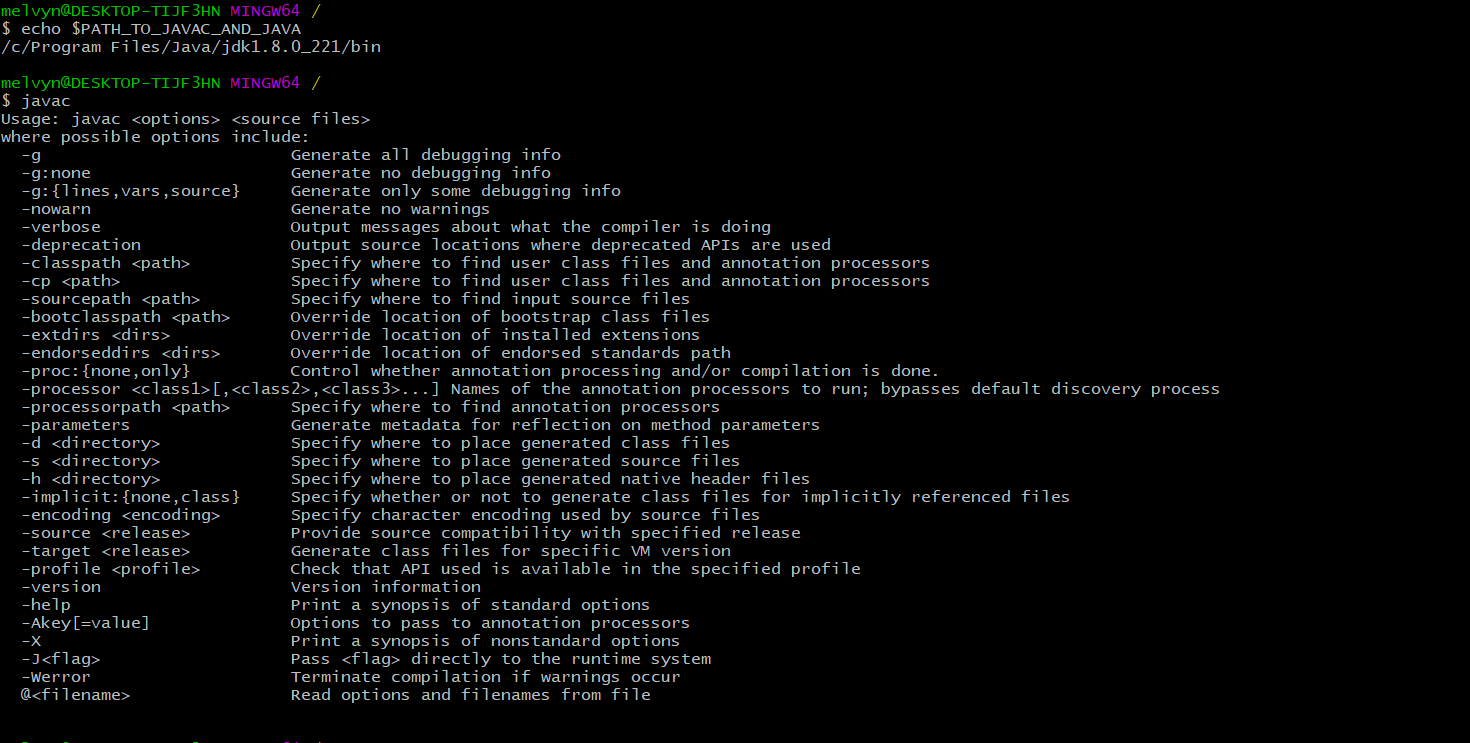
\includegraphics[width=0.9\textwidth]{Images/works.PNG}
  \caption{All set up and ready to go.}
	\label{errorisokay}
\end{figure}

\subsection{Compile a simple program}
So part 1 of your exam is to configure your PATH and you've now done it. Part 2
of your exam is to write and compile a standard foobar program. This is a
standard first interview question that verifies that you understand the absolute
basics of a programming language and can implement a simple concept in the
language. The problem statement is:

Write a program that will loop over the numbers from 1 to 100 ( inclusive) and
generate the following outputs:

\begin{center}
\begin{itemize}
\item if i is a multiple of 3 print foo on a line.
\item if i is a multiple of 5 print bar on a line.
\item if i is a multiple of 15 ( both 3 and 5 ) print foobar on a line.
\end{itemize}
\end{center}

For example, if you run the code from i = 1 to 15 instead of 1 to 100 you should
get the following output:

\begin{lstlisting}[language=Bash]
melvyn@gitbash$ java foobar
foo
bar
foo
foo
bar
foo
foobar
\end{lstlisting}

 where the outputs correspond to 3, 5, 6, 9, 10, 12, 15. Your final exam is to
set up your PATH on an NJCU machine, then write, compile and run a foobar
program and get the right answer.

{\LARGE\textbf{In class activity}}

\begin{center}
{\LARGE Figure out what the output should be as a class. Write it on the board.
Pretty easy stuff. It's up to the students to write the code, but we can
determine the output together. }
\end{center}

\section{Grading for Final}
You must do the exam on an NJCU machine. The computer will not have internet
connectivity and I'll be logging all your keystrokes to verify it's you doing
the work. This is why we have to do it on an NJCU machine. When we come next
week I expect you here on time at 8:00 - we'll be done at 8:30 sharp, make sure
you are here on time and ready to do the assignment. Get it done, get 50 pts for
the path, 50 pts for the code. Get an A, please!!!!

This has been a hard semester, let's finish on a high note with a bunch of good
grades.

\section{Graphing in Java}
This is a project I had intended to do with you but didn't prepare because there
was no time for us to do it. 

Give 20 points extra on midterm if you submit some compileable code that uses
JCommon and JFreeChart to plot the coordinates in the dinosaur from the
dinosaurus dozen dataset.
\subsection{Datascience}
there is no reason you CANT do great datascience in Java. Java is a powerful
language like so many others - it's just that Python, R and Scala have sort of
take over the domain. Anyway, we're learning Java and I like math, so I've
wanted to do a graphing project for this class. Since we have time now in our
last lecture let's try it.
\end{document}

